\chapter{Анализ существующих подходов к статическому анализу, проектирование архитектуры и
исследование средств реализации}

\section{Виды структур представления информации в статическом анализе}

Из подраздела \ref{ssec:2:results} становится ясно, что в отношении мультиязыкового анализа
основополагающим механизмом является наличие общей структуры представления информации, позволяющей отражать различные
сущности различных языков в единой форме. Выбор такой структуры может влиять на следующие
характеристики метода анализа:
\begin{itemize}
    \item разнообразие поддерживаемых языков,
    \item сложность разработки и поддержки анализаторов,
    \item корректность и полнота анализа,
    \item возможные сценарии использования.
\end{itemize}
В целом, выбор структуры влияет практически на все характеристики метода, поэтому стоит
исследовать существующие структуры представления информации о программном коде.

AST \Abbrev{AST}{abstract syntax tree --- абстрактное синтаксическое дерево}
 представляет собой репрезентацию программного кода в древовидном формате. В качестве узлов дерева выступают различные синтаксические конструкции, а в качестве ребер связи между ними. AST является
простой и универсальной структурой данных, позволяющей реализовывать множество анализов. Также,
носителем AST может быть любой структурный формат (например S-выражения), что упрощает его
построение, сериализацию и анализ. Однако, в контексте мультиязыкового анализа AST является
неудобным решением, в первую очередь потому что оно часто вовлекает языкоспецифичные конструкции.
К примеру, в некоторых языках отсутствует понятие <<оператор>> (англ statement), что различает
AST таких языков от императивных языков на фундаментальном уровне.

eCST \cite{eCST} является попыткой расширения концепции AST (а точнее CST \Abbrev{CST}{concrete syntax tree --- частное синтаксическое дерево}) на большее
количество языков. Авторы достигают этого путем введения универсальных узлов, позволяющих
отражать общие семантические концепции (итерацию, выбор или переход). К сожалению, такой формат
представления информации всё еще неудобен так как языкоспецифичные узлы не могут быть конвертированы
в такие универсальные узлы и остаются в дереве в первозданном виде.

CFG \Abbrev{CFG}{control flow graph --- граф потока управления} это граф, узлы которого представляют собой в общем случае операторы, а ребра
поток управления. Такой граф полезен в первую очередь для компиляторных трансформаций и оптимизаций,
так как позволяет моделировать исполнение программы и выстраивать на основе этого определенные инварианты.
Граф является основой для фреймворков монотонного анализа \cite{static-program-analysis} и активно
используется в различных инструментах. Несмотря на достоинства, как и в случае с AST такой граф
имеет зависимость от представляемого языка. Также, анализ потока управления сложен в контексте
мультиязыкового статического анализа и проще осуществим в рамках динамического анализа.

CDG является формой представления информации о вызовах процедур друг другом в контексте
определенного фрагмента кода. Соотвественно, узлы такого графа обычно составляют идентификаторы
процедур, а ребра зависимость <<вызывает>>. Стоит сказать, что зависимость <<вызывает>> обычно является
направленной, поэтому граф имеет направление ребер. Такой граф является хорошим кандидатом на универсальное
представление в рамках мультиязыкового анализа, что уже было исследовано \cite{MLSA}. Как было
сказано в подразделе \ref{ssec:mlsa}, основным недостатком графа зависимостей вызовов является
его ориентированность на процедуры -- исполняемые фрагменты кода. Это делает невозможным его применение
в рамках других языков, в первую очередь форматов данных. Действительно, в современных приложениях
семантически важная информация часто содержится в различных конфигурационных файлах, например XML или
INI.

Система типов обычно не является ни структурой данных ни моделью представления семантической информации.
Её основное назначение заключается именно в проверке программ на определенные классы ошибок,
что достигается путем задания определенного набора суждений о сущностях в программе с
их дальнейшей автоматической проверкой.
Однако, современные исследования в области системы типов показывают, что
есть возможность кодирования и эффективной проверки ряда свойств программного кода, часть
которых раньше могла быть проверена только интенсивным статическим анализом. Примером является
механизм borrow-checking в языке Rust \cite{rust}, который базируется на системе типов известной
как система \textit{владения}. Такой механизм позволяет проверять и устранять класс ошибок связанных
с системными ресурсами: использование после освобождения, предотвращенние гонок данных и другие.
В контексте мультиязыкового анализа система типов точно имеет первостепенное значение, так
как создание корректных анализаторов возможно в том числе за счет использования корректной
системы типов. Однако, одной системы типов для совершения анализа недостаточно, так как
обычно ограничения на типы сущностей не берут в расчет механизмы областей видимости языков
и семантику зависимостей сущностей между собой.

Таблица символов является повсеместной структурой данных (особенно в императивных языках) и
используется в первую очередь для представления различной информации об идентификаторах. Так,
таблица символов обычно содержит данные о местонахождении определения (или объявления) сущности,
её тип, контекст в котором она определена и множество других атрибутов, специфичных для конкретного
языка. Структурно таблица символов представляет собой набор пар (идентификатор, атрибуты).
Первым и значимым расширением концепции таблицы символов является введение понятия \textit{области видимости}.
В языках с лексической областью видимости таблица символов является не таблицей, а стеком таблиц --
это необходимо для отражения отношения вложенности между областями видимости. Таблица символов
является очень хорошим решением в контексте мультиязыкового анализа, но имеет один серьезный недостаток.
Он заключается в отсутствии возможности однозначного кодирования нелексических
областей видимости, например в случае присутствия в языке механизма классов или модулей.

Граф свойств может быть определен в терминах теории графов как направленный 
мультиграф с метками вершин и ребер с собственными ребрами, 
где ребра имеют собственную идентичность \cite{property-graph}.
Такие графы активно используются в графовых базах данных и хорошо подходят для отражения
разноструктурированной онтологической информации о сущностях в области знаний.
Например, формат RDF \cite{RDF} является основным способом представления информации
в семантических сетях Интернета. Основанные на нем языки отражения онтологических
понятий позволяют создавать машинно-читаемые семантические структуры.
Основным недостатком графов свойств в контексте мультиязыкового анализа ПО является отсутствие
сколько нибудь универсальной единой онтологической модели. Соотвественно, существующие
модели (что рассмотрены в подразделе \ref{ssec:pangea}) являются специфичными решениями.
Также, создание и поддержка таких моделей является довольно трудоемким процессом, так как требует
достаточной компетенции специалиста.

Таким образом, на данный момент не существует идеальной структуры представления информации
для осуществлений мультиязыкового анализа. Однако, существующие структуры и модели дают
представление о том, какой она могла бы быть -- идеальная модель являлась бы совмещением
концепций системы типов и таблицы символов, с дополнительной возможностью связывания
понятий по онтологическим признакам в определенные графы свойств. Таким образом, так или иначе
такая модель должна реализовывать формат семантической сети в общем случае.

\section{Архитектура метода анализа} \label{sec:architecture}

\subsection{Парсинг мультиязыковых фрагментов кода}

Как было сказано в подразделе \ref{ssec:parsing-problem}, парсинг текста является одной из первых
задач, которые необходимо решить при мультязыковом анализе. При наличии единой модели представления информации,
однако, такая задача существенно упрощается.

Дело в том, что используя единую модель состоящую из графа можно достичь разделения этапов
извлечения информации о графе и анализа самого графа. Похожий подход используется, например, при
реализации проверки типов методом Хиндли-Милнера \cite{algorithm-W}. Суть алгоритма заключается
в использовании т.н. \textit{ограничений} которые извлекаются из кода. Такие ограничения являются
утверждениями о сущностях и в дальнейшем решаются вместе для создания специальной подстановки, которая
позволит удовлетворить все ограничения. Такой процесс решения называется \textit{унификацией}.

По тому же принципу можно построить модель для мультиязыкового анализа, если в качестве ограничений
воспринимать отношения узлов в графе, а в качесте процесса унификации процесс построения самого графа. Такой
механизм распределенного анализа позволяет достичь трех целей:
\begin{itemize}
    \item разделение метода на два этапа (генерация ограничений и их разрешение), что повышает
    модульность анализатора, его универсальность и открывает возможности для параллелизации,
    \item объединение анализаторов таким представлением как ограничения позволяет решить проблему
    парсинга мультиязыковых фрагментов путем реализации специализированных (заточенных под конкретный
    язык) анализаторов,
    \item открываются возможности для реализации инкрементального анализа и анализа неполного графа, что
    критично для таких средств как IDE и линтеры.
\end{itemize}

Таким образом, такие анализаторы являются \textit{трансляторами} из избранного языка в унифицированное представление,
заданное в виде ограничений.

Стоит заметить, что создание раздельных трансляторов под конкретный язык всё еще не решает проблему
взаимодействия языков в общем случае, так как часто в коде на избранном языке встречаются фрагменты
кода, реализованные на других языках. Обычно, такой код представляется строковым литералом. К примеру,
фрагменты такого <<встроенного>> кода могут включать:
\begin{itemize}
    \item путь к файлу или ресурсу (в формате URI),
    \item данные в определенном формате (например XML, JSON...),
    \item строка запроса к БД (например SQL),
    \item шаблон документа или веб страницы (в формате HTML),
\end{itemize}

Такие фрагменты в общем случае сложно обнаружить в исходном коде так как строковые литералы
могут быть представлены в любом выражении. Решением данной проблемы может служить инструмент
распознавания определенного языка программирования по входной строке. Таким образом,
трансляция определенного языка будет вовлекать распознавание фрагментов языков, описанных через строковые литералы.
После распознавания такие фрагменты будут направлены соответствующим трансляторам.

Таким образом, общий алгоритм трансляции выглядит следующим образом:
\begin{enumerate}[1)]
    \item на вход транслятору поступает фрагмент кода на определенном языке,
    \item транслятор использует любые подходящие средства для анализа и трансляции данного кода
    (AST, CFG, абстрактная интерпретация и т.д.),
    \item если транслятор обнаруживает строковый литерал он может отправить его на распознавание, которое
    позволит определить язык избранного фрагмента и в дальнейшем направить этот фрагмент другому транслятору,
    \item все трансляторы всех языков выводят ограничения в общий буфер, для последующего разрешения.
\end{enumerate}

Как видно из алгоритма, универсальное представление позволяет реализовывать гибкий анализ кода --
сам процесс анализа зависит от конкретного транслятора и может вовлекать любые методы, вплоть до интерпретации
или компиляции. Также такая трансляция происходит независимо от остальных трансляторов, что
позволяет проводить анализ проектов инкрементально и по требованию.

\subsection{Унифицированное представление через ограничения} \label{ssec:constraints-desc}

В ходе работы над проектом были реализованы несколько представлений, способных быть достаточно универсальными
и при этом распределенными. Были рассмотрены такие структуры как семантическая сеть и дерево модулей, однако
такие представления ориентированы на другие сценарии использования, поэтому их корректная
адаптация под статический анализ затруднительна. Однако, общей идеей в обоих структурах было 
создание графа \textit{идентификаторов}, каждый из которых обладал бы одной из двух
семантик: либо \textit{объявление}, либо \textit{ссылка}.

Объявлением называется семантика создания имени ресурса. Если при этом ресурс привязывается к такому имени, то
такое действие называется определением. Ссылкой же называется дальнейшее упоминание такого имени в тексте
программы. В контексте мультиязыкового статического анализа данную семантику можно понимать следующим образом.

Объявлением является идентификатор, находящийся в определенном фрагменте кода определенного языка и факт того, является
ли идентификатор объявлением определяется транслятором этого языка. Ссылкой является идентификатор находящийся \textit{в
другом фрагменте кода, реализованным на другом языке}. Факт того, что идентификатор является ссылкой тоже определяется
транслятором избранного языка. Таким образом создается набор идентификаторов, определенные из которых можно сопоставить друг
с другом, получив таким образом пары (объявление, ссылка).
Эта базовая идея позволяет обнаруживать различные межъязыковые связи различной природы, так как на вид самого идентификатора
не налагается никаких ограничений -- это может быть URI файла, имя функции, имя модуля или ключ в БД.

Однако, современные проекты в подавляющем большинстве случаев структурированы с учетом изоляции имен. Такой механизм
обычно называется механизмом \textit{областей видимости}. Описанная выше схема пренебрегает таким механизмом, что
ведет в сущности к лексическому сопоставлению идентификаторов, который не обладает ни должной корректностью, ни полнотой.

Учитывая, что понятие области видимости тесно связано с понятием <<модуль>> (так как последний часто определяется
как именованная область видимости с возможностью импорта),
логичным решением является использование универсальной системы модулей для организации идентификаторов в области
видимости. Одной из таких систем может являться механизм \textit{графов областей видимости} \cite{scope-graphs}.
Графы областей видимости (далее просто графы областей) являются языконезависимой теорией описания таких
механизмов как привязка имен и их разрешение. В оригинальной статье авторами создается соответствующий граф,
узлами которого могут выступать идентификаторы и области видимости, а ребрами -- различные отношения между ними. В граф входят
такие бинарные отношения как:
\begin{itemize}
    \item объявлен в,
    \item имеет ссылку в,
    \item должен быть разрешен в,
    \item родительская область видимости,
    \item достижим,
    \item видим,
\end{itemize}

Как видно из списка, данные отношения позволяют задавать богатую семантику разрешения имен, при этом
не используя понятия определенного языка программирования. Авторам удается реализовать семантику
импорта и включения модулей, а также структуру лексических областей видимости.

Данный фреймворк хорошо подходит для данной задачи, однако в дальнейшем авторами оригинальной статьи
был создан другой, более подходящий для статического анализа фреймворк. В статье \cite{scope-graphs-static-analysis}
описывается метод генерации графа областей через использование ограничений, ориентированный на реализацию
статических анализаторов. Интерес в первую очередь представляют результаты работы авторов -- им удалось
существенно упростить фреймворк и включить более универсальные отношения в граф, за счет чего им удается увеличить
количество информации, которую можно представить таким графом. 

Основным изменением по сравнению с оригинальной работой 2015 года, однако, стало введение типов. В смежной работе
\cite{scope-graphs-typed} авторами рассмотрен механизм графов областей в для которого вводится еще один тип
ограничений -- ограничения на типы идентификаторов. Такой подход позволяет реализовать \textit{смешанное} разрешение
имен, когда процесс разрешения вовлекает как поиск идентификатора в графе, так и вывод типа. Основной причиной
введения такого механизма стало использование таких языковых конструкций как записи. В отличие от модулей, записи
могут иметь экземпляры, то есть в процесс разрешения поля записи вовлекается процесс разрешения типа экземпляра переменной.

Стоит заметить очень важную особенность фреймворка -- авторами тщательно доказываются все заявленные свойства
через задание формальной семантики. Таким образом обеспечивается корректность алгоритма разрешения имен с учетом
изложенного исчисления. Это очень важное свойство, отличающее фреймворк авторов и, соответственно, данный метод,
так как корректность позволяет создавать более надежные и точные средства автоматизированного анализа.

В качестве базы модели разрабатываемого метода анализа используется граф областей видимости в редакции статьи \cite{scope-graphs-static-analysis}
, то есть задаваемый через ограничения. В отличие от графа описанного в \cite{scope-graphs-typed},
данный граф имеет более простую организацию и не вовлекает отношение подтипирования. Помимо ограничений, собираемых
в ходе построения графа областей и анализа типов идентификаторов решено было ввести дополнительные виды ограничений,
позволяющих обеспечивать проверку дальнейшую корректности связей в проекте. Ниже перечислены все задействованные
в методе анализа виды ограничений:

\renewcommand{\labelenumi}{\arabic{enumi})}
\renewcommand{\labelenumii}{\asbuk{enumii})}

\begin{enumerate}
    \item Объявление\slash Ссылка,
        \begin{enumerate}
        \item \textbf{Вид:} ограничение графа областей;
        \item \textbf{Вовлекаемые узлы:} область видимости в которой упомянут идентификатор, идентификатор;
        \item \textbf{Назначение:} связывание идентификатора и области видимости.
        \end{enumerate}
    \item Прямое ребро,
    \begin{enumerate}
        \item \textbf{Вид:} ограничение графа областей; 
        \item \textbf{Вовлекаемые узлы:} две области видимости, наименование ребра;
        \item \textbf{Назначение:} обозначение прямой связи
        между областями, моделирование лексических областей видимости.
    \end{enumerate}
    \item Ассоциация,
    \begin{enumerate}
        \item \textbf{Вид:} ограничение графа областей;
        \item \textbf{Вовлекаемые узлы:} идентификатор или переменная, область видимости;
        \item \textbf{Назначение:} <<именование>> определенной
        области видимости, либо указание того что данный идентификатор имеет привязанную область видимости.
    \end{enumerate}
    \item Разрешение,
    \begin{enumerate}
        \item \textbf{Вид:} ограничение графа областей;
        \item \textbf{Вовлекаемые узлы:} идентификатор, идентификатор или переменная;
        \item \textbf{Назначение:} указание того что
        данный идентификатор должен быть разрешен либо в указанный идентификатор, либо в подстановку переменной.
    \end{enumerate}
    \item Уникальность,
    \begin{enumerate}
        \item \textbf{Вид:} ограничение графа областей;
        \item \textbf{Вовлекаемые узлы:} коллекция имен;
        \item \textbf{Назначение:} указание что коллекция имен не содержит дубликатов
        в рамках данной области видимости.
    \end{enumerate}
    \item Подмножество,
    \begin{enumerate}
        \item \textbf{Вид:} ограничение графа областей;
        \item \textbf{Вовлекаемые узлы:} две коллекции имен;
        \item \textbf{Назначение:} указание того, что одна коллекция
        имен входит в другую коллекцию имен.
    \end{enumerate}
    \item Аннотация типа,
    \begin{enumerate}
        \item \textbf{Вид:} типовое ограничение;
        \item \textbf{Вовлекаемые узлы:} идентификатор, переменная;
        \item \textbf{Назначение:} указание типа определенного
        идентификатора через переменную.
    \end{enumerate}
    \item Равенство типов,
    \begin{enumerate}
        \item \textbf{Вид:} типовое ограничение;
        \item \textbf{Вовлекаемые узлы:} две переменные;
        \item \textbf{Назначение:} обозначение равенства друх типовых 
        переменный для их последующей унификации.
    \end{enumerate}
    \item Обязан разрешиться,
    \begin{enumerate}
        \item \textbf{Вид:} ограничение консистентности;
        \item \textbf{Вовлекаемые узлы:} идентификатор, область видимости;
        \item \textbf{Назначение:} наложение на ссылку ограничения, обязывающего дальнейшее
        связывание с объявлением.
    \end{enumerate}
    \item Необходимый,
    \begin{enumerate}
        \item \textbf{Вид:} ограничение консистентности;
        \item \textbf{Вовлекаемые узлы:} идентификатор, область видимости;
        \item \textbf{Назначение:} данное объявление должно иметь хотя бы одну ссылку.
    \end{enumerate}
    \item Эксклюзивный,
    \begin{enumerate}
        \item \textbf{Вид:} ограничение консистентности;
        \item \textbf{Вовлекаемые узлы:} идентификатор, область видимости;
        \item \textbf{Назначение:} данное объявление должно иметь не более одной ссылки.
    \end{enumerate}
    \item Знаковый,
    \begin{enumerate}
        \item \textbf{Вид:} ограничение консистентности;
        \item \textbf{Вовлекаемые узлы:} идентификатор;
        \item \textbf{Назначение:} данное объявление может встречаться только
        в одном экземпляре во всем графе областей видимости.
    \end{enumerate}
\end{enumerate}

Дополнительные виды ограничений консистентности (<<Обязан разрешиться>>, <<Необходимый>>, <<Эксклюзивный>>, <<Знаковый>>) не затрагивают
оригинальный механизм разрешения имен в графе областей и являются простым расширением, позволяющим добавить
дополнительную информацию для инструментального средства. Такая информация будет интерпретироваться только
им и не будет иметь влияния на процессы построения и решения графа.

\subsection{Вовлечение операционного окружения}

Текущее описание метода предполагает однонаправленное взаимодействие с инструментальным средством -- метод,
получая данные для анализа, проводит трансляцию и решение ограничений, предоставляя результаты в виде решенного
графа и других ограничений.

Однако, для практической реализации метода неизбежно придется ответить на следующие вопросы:
\begin{enumerate}[1.]
    \item Как будет происходить выборка кода для анализа?
    \item Каким образом будет учитываться окружение проекта?
\end{enumerate}
Стоит рассмотреть каждый вопрос в отдельности.

Выборка кода для анализа является сложной в общем случае задачей, так как подразумевает
промежуточный анализ некоторых файлов проекта и его окружения для получения необходимых
путей к файлам кода. Поэтому, извлечение кода в данном методе делегируется конкретному инструментальному
средству. Это позволяет достичь следующих целей:
\begin{itemize}
    \item упрощение метода анализа,
    \item облегчение поддержки специфических сценариев сборки и кодогенерации,
    \item повышение универсальности метода анализа.
\end{itemize}

Данное обособление метода является логичным, так как каждое конкретное инструментальное
средство может быть заинтересовано в разных объемах кода и в разных его характеристиках.

Однако, для обеспечения полноценного анализа имеет смысл использовать операционное окружение
проекта. Включение в граф областей такой информации может упростить сценарии анализа
языков сборки и оболочки командной строки.
Для анализа операционного окружения проекта предполагается отображение такого рода информации в виде
явных данных в формате ограничений. Таким образом, появляется компонент \textit{провайдер конфигурации}.
Он ответственен за отображение данных об операционном окружении в формат ограничений перед
этапом трансляции избранных языков. С его помощью могут быть выражены следующие данные об окружении:
\begin{itemize}
    \item содержимое файловой системы (через граф областей),
    \item имена и тип различных системных переменных (через ограничения типизации),
\end{itemize}

Таким образом, возможна реализация анализа <<над>> разными языками программирования, так как
 вовлекается анализ внешнего мира, в котором они взаимодействуют. Это позволяет
 покрыть большую часть сценариев использования метода анализа в контексте различных
 инструментальных средств. 

Стоит также заметить, что информация об источнике определенного ограничения может быть полезна для использования
в инструментальных средствах при интерпретации этих решенных ограничений. Поэтому для каждого ограничения также вводится
поле об источнике -- пара из пути к файлу/фрагменту и названия языка на котором написан фрагмент. Такой
подход также позволяет установить \textit{границы} между модулями на различных языках, что может быть полезно
для определенных проектов. Такие границы позволяют уменьшить количество ложноположительных результатов, если
известно что определенная пара языков никак не должна взаимодействовать и между фрагментами таких языков не может быть
междъязыковых связей. 

Примером может служить пара из языка для написания документации(например Markdown) и другого языка программирования.
Обнаружение таких межъязыковых связей может быть нежелательно для разработчика инструментального средства и
избежать этого можно путем последующей интрепретации решенных ограничений с учетом межъязыковых границ.

\subsection{Онтология} \label{ssec:ontology}

Онтологией обычно называется набор определенных знаний о предметной области.
Однако, в контексте данной работы такой термин будет использоваться для иных целей -- им будет
обозначаться набор механизмов, позволяющих \textit{обеспечивать консистентность} между различными
трансляторами различных языков. Такое название для группы данных механизмов было выбрано
в первую очередь для сохранения изначального смысла определения -- вне зависимости от того,
каким образом онтология может быть реализована (например, как набор механизмов сохранения консистентности),
она в любом случае несет в себе важную информацию о предметной области.

Таким образом, с практической точки зрения онтология реализуется через создание двух компонентов:
\begin{itemize}
    \item типового контекста,
    \item верификатора структуры подграфа.
\end{itemize}

Типовый контекст содержит все данные для организации <<настраиваемой>> системы типов над графом областей.
Например, в исходной работе \cite{scope-graphs-typed}
представлена более широкая система типов в сравнении с \cite{scope-graphs-static-analysis} так как помимо прочего включает
механизм подтипирования. Таким образом, в типовый контекст входят обычные типы (англ. ground types), типовые конструкторы
(например, функциональная стрелка или тип-произведение) и дополнительные конструкции избранной системы типов (например, отношения подтипирования).

Стоит заметить, что такой гибкий подход к системе типов позволяет создавать довольно мощные механизмы разрешения имен. Например,
появляется возможность связывания объявлений и ссылок не только по именам, но и по \textit{значениям}. Этого можно достичь, используя
механизм типов пересечений и типов объединений \cite{DEZANICIANCAGLINI1992303}.
Расширив систему типов таким образом, можно будет присвоить идентификатору сильно ограничивающий тип. В качестве примера можно рассмотреть
исходный код на языке TypeScript:
\begin{minted}[linenos=true]{ts}
    const a: 1 | "a" = 1
    const b: 1 | "a" = "a"
    const c: 1 | "a" = true
\end{minted}

В данном случае определение типа \texttt{1 | "a"} указывает, что идентификатор с такой типовой аннотацией может быть
привязан либо к значению 1, либо к строке \texttt{"a"}. Таким образом, строка 3 считается ошибочной и в контексте
разрешения имен это значит, что такое имя никогда не будет связано с переменной иного типа. Такой подход позволяет
сильно упростить некоторые сценарии наложения ограничений (например, когда необходимо показать что идентификатор всегда связывает
определенное значение и оно известно наперед).

В современной индустрии используется большое количество ООП языков: Java, Kotlin, C\#, PHP, TypeScript и многие другие.
Хотя концепция \textit{класса} и \textit{объекта} примерно одинакова во всех языках, строгого соответствия между
языками всё же нет. К тому же, в разных языках одинаковые синтаксически определения могут очень сильно отличаться по
семантике. Например, объект класса в Java всегда будет сравниваться с другим объектом номинально, хотя
в TypeScript такой же (синтаксически) объект может участвовать в структурном сравнении.

Этот факт, а еще факт того, что концепция модулей в языках программирования в целом тоже довольно сильно
отличается от языка к языку, вынуждает разработчика транслятора определенного языка учитывать очень
специфические языковые концепции. Такой подход неизбежно ведет к ограничению количества поддерживаемых в анализе языков
и переусложнению модели анализа.
Именно поэтому метод мультиязыкового анализа должен поддерживать максимально
обобщенное представление -- оно позволяет кодировать различную языковую семантику в единой и краткой форме. Но в таком случае
появляется проблема согласованности -- специфические конструкции одного языка могут быть представлены не так, как конструкции иного языка, но
семантически они могут значить одно и то же. Эта проблема \textit{неизбежна}, так как мультиязыковой анализ
 вовлекает многие независимые трансляторы (на каждый язык), каждый из которых может быть разработан создан любым разработчиком. 

Для решения данной проблемы предполагается использование механизма \textit{структурной верификации}. Ограничения, помимо прочего,
задают набор \textit{известных фактов}. Эти факты являются начальными данными для алгоритма разрешения имен. Именно
такие факты должны быть согласованны между трансляторами для того чтобы семантика классов и модулей различных языков
была отражена единообразно, так как это позволяет производить верное разрешение имен в дальнейшем. Для обеспечения такой
согласованности можно осуществлять верификацию структуры ограничений на этапе их генерации.

В качестве примера работы такого механизма можно рассмотреть следующий код на C\# взятый из примера проекта на платформе dotnet \cite{eShopOnWeb}:

\begin{minted}[linenos=true, breaklines]{csharp}
    [ApiExplorerSettings(IgnoreApi = true)]
    [Authorize]
    [Route("controller/action")]
    public class OrderController : Controller
    {
        private readonly IMediator _mediator;
    
        public OrderController(IMediator mediator)
        {
            _mediator = mediator;
        }
    
        [HttpGet]
        public async Task<IActionResult> MyOrders()
        {   
            Guard.Against.Null(User?.Identity?.Name, nameof(User.Identity.Name));
            var viewModel = await _mediator.Send(new GetMyOrders(User.Identity.Name));
    
            return View(viewModel);
        }
    
        [HttpGet("{orderId}")]
        public async Task<IActionResult> Detail(int orderId)
        {
            Guard.Against.Null(User?.Identity?.Name, nameof(User.Identity.Name));
            var viewModel = await _mediator.Send(new GetOrderDetails(User.Identity.Name, orderId));
    
            if (viewModel == null)
            {
                return BadRequest("No such order found for this user.");
            }
    
            return View(viewModel);
        }
    }
\end{minted}

Вышеприведенный класс имеет большое количество различных аннотаций (как в определении класса, так и в определении
методов). Также, он наследует от класса \texttt{Controller}. Однако, на уровне межъязыковых связей, можно
сказать что этот класс является одним из эндпоинтов веб-сервера, который выполняет различные действия по различным
HTTP запросам (в данном примере это GET запросы). Разработчику моноязыкового транслятора хотелось бы каким-либо образом извлечь эту информацию
в формальной форме и структура самого класса в контексте межъязыкового анализа для него
неинтересна. Для этого хорошо подходит структура задаваемая ограничениями, но они являются слишком абстрактным представлением
и не поддерживают идею <<абстрактного веб-сервера>> напрямую. Тогда, может быть разработан набор правил верификации
структуры веб-сервера (приведенных неформально):
\begin{enumerate}[1)]
    \item имеет ли модуль название \texttt{WebServer},
    \item имеет ли он поле \texttt{GET} которое тоже является модулем,
    \item имеет ли такой модуль поле \texttt{application/json}, 
    \item имеет ли такое поле схему json (иерархическую структуру, имеющую типы JSON),
    \item имеет ли модуль \texttt{WebServer} поле \texttt{POST},
    \item и другие возможные проверки...
\end{enumerate}

Таким образом, извлекаемые транслятором ограничения могут быть проверены на соответствие такому <<архетипу>> веб-сервера.
Если ограничения не имеют такую структуру, то транслятор потерял согласованность с другими трансляторами и должен быть доработан.

В итоге, механизм верификации структуры позволяет достичь следующих целей:
\begin{enumerate}[1)]
    \item упрощение поддержки мультиязыкового транслятора и согласованности моноязыковых трансляторов,
    \item поддержка более сложных семантических конструкций на основе классов и модулей (веб-сервер, библиотека, графический ресурс и многие другие),
    \item облегчение модели анализа с расширенной поддержкой языко-специфичных конструкций (если они выражаемы через механизм классов или модулей).
\end{enumerate}

Подводя итоги подраздела \ref{sec:architecture}, можно составить общую диаграмму потока данных между вовлеченными модулями. Такая
диаграмма представлена на рисунке \ref{fig:framework}.

\begin{figure}[H]
    \centering
    \resizebox{1.05\linewidth}{!}{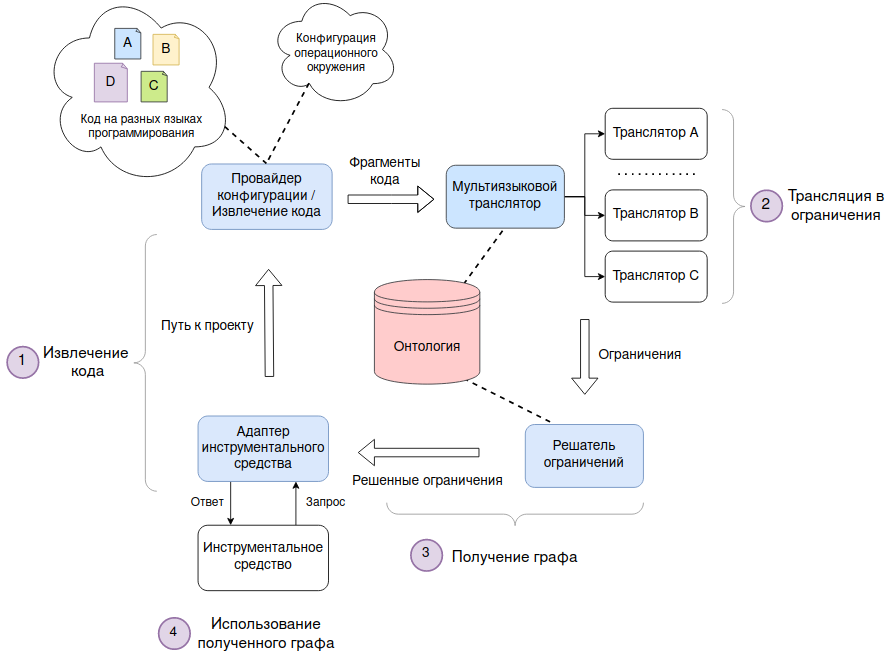
\includegraphics[height=0.85\textheight]{inc/img/framework}}
    \caption{Структура метода в виде диаграммы потока данных}
    \label{fig:framework}
\end{figure}

\section{Исследование средств реализации}

Учитывая поставленные задачи
логичным решением было выбрать популярный формат данных, который хорошо поддерживается современными
языками. В качестве основного формата передачи (т.е. носителем) ограничений решено было выбрать JSON.
Он является универсальным форматом структурированных данных, используемым в большом количестве
различных технологий и инструментов. В данном случае, формат был выбран по следующим причинам:
\begin{itemize}
    \item простота и универсальность,
    \item широкая поддержка в различных языках и средствах,
    \item относительная компактность,
    \item частая интеграция формата в существующих инструментальных средствах.
\end{itemize}

В целом язык не является основополагающим при разработке анализатора, так как не требуется
никаких специфических технологий для его реализации. При разработке в рамках данной работы
было решено выбрать язык Golang. Это прикладной императивный язык, поддерживающий
компиляцию в машинный код и небольшой рантайм, при этом сопровождая большинство
удобных функциональных возможностей для упрощения процесса разработки.
Из плюсов языка в контексте данного проекта можно отметить следующие особенности:
\begin{itemize}
    \item простота синтаксиса и семантики,
    \item наличие статической типизации,
    \item относительно легкая работа с динамическими (как JSON) данными,
    \item большое количество различных библиотек и очень высокое качество средств поддержки разработчика,
    \item быстрая компиляция и высокое быстродействие программ.
\end{itemize}

Минусами языка выступают: ограниченная система типов, слабая поддержка нетривиальных подходов к решению задач,
сильный расчет на динамические проверки во время исполнения.
Однако, для данного проекта эти минусы несущественны и не помешают реализации
основных модулей анализатора.
\clearpage